\documentclass[14pt,a4paper]{article}

\usepackage[utf8]{inputenc}

\usepackage{amssymb}

\usepackage{amsfonts}


\usepackage{graphicx}

\usepackage[left=3cm,right=3cm,top=3cm,bottom=3cm]{geometry}

\date{\today}


\begin{document}
\title{Comunicación para el desarrollo del proyecto}


\includegraphics[scale=0.4]{uv1.png} 
\author{Equipo 1}


\section{Objetivos}
\begin{itemize}
\item \textit{Establecer los distintos roles.}
\item \textit{Cumplir con los objetivos establecidos para éste proyecto.}
\item \textit{Establecer reglas para el trabajo en equipo}
\item \textit{Una comunicación éxitosa entre los miembros del equipo.}
\item \textit{Realizar llamadas para aclarar dudas.}
\end{itemize}
\vspace{0.7 cm} 



\section{Plan de comunicación}
\vspace{0.5 cm}
\begin{verse}
Para el desarrollo de este proyecto decidimos utilizar Discord; La razón por la cual nuestro equipo decidió ocupar Discord y no otra aplicación es porqué Discord es un programa que es completamente gratuito, que tiene una latencia bastante baja, consume muy pocos recursos, es seguro, se pueden crear canales muy similares a un foro, agregar a miles de personas, tener conversaciones en dichos canales por texto La importancia de la comunicación radica en que es nuestro medio para entendernos los unos a los otros, es nuestra herramienta para conseguir lo que necesitamos y lo que queremos, así cómo lo que somos. 
Para el desarrollo de éste proyecto tuvimos la necesidad de asignar roles, y en Discrod es posible otorgar diferentes roles a cada miembro. También cuenta con una app disponible para dispositivos móviles la cual no se encuentra limitada y se puede hacer todo lo que podrías hacer en un ordenador. Las opciones de configuración de la app te permiten modificarlas como desees hasta para que consuma menos recursos y menos conexión a internet manteniendo la calidad del audio en todo momento.
Al utilizar una herramienta de comunicación con la que todos los integrantes del equipo estaban familiarizados, fue más sencillo la distribución, así como la creación del proyecto. La elección de la plataforma adecuada jugó un papel importante en el desarrollo del proyecto, ya que gracias a ello pudimos programar nuestras reuniones, así como también dar una retroalimentación a quien tuviera alguna duda. Todos los días nos contactábamos para mantener al tanto de nuestro progreso a todos los integrantes del equipo.
\begin{figure}[htb]


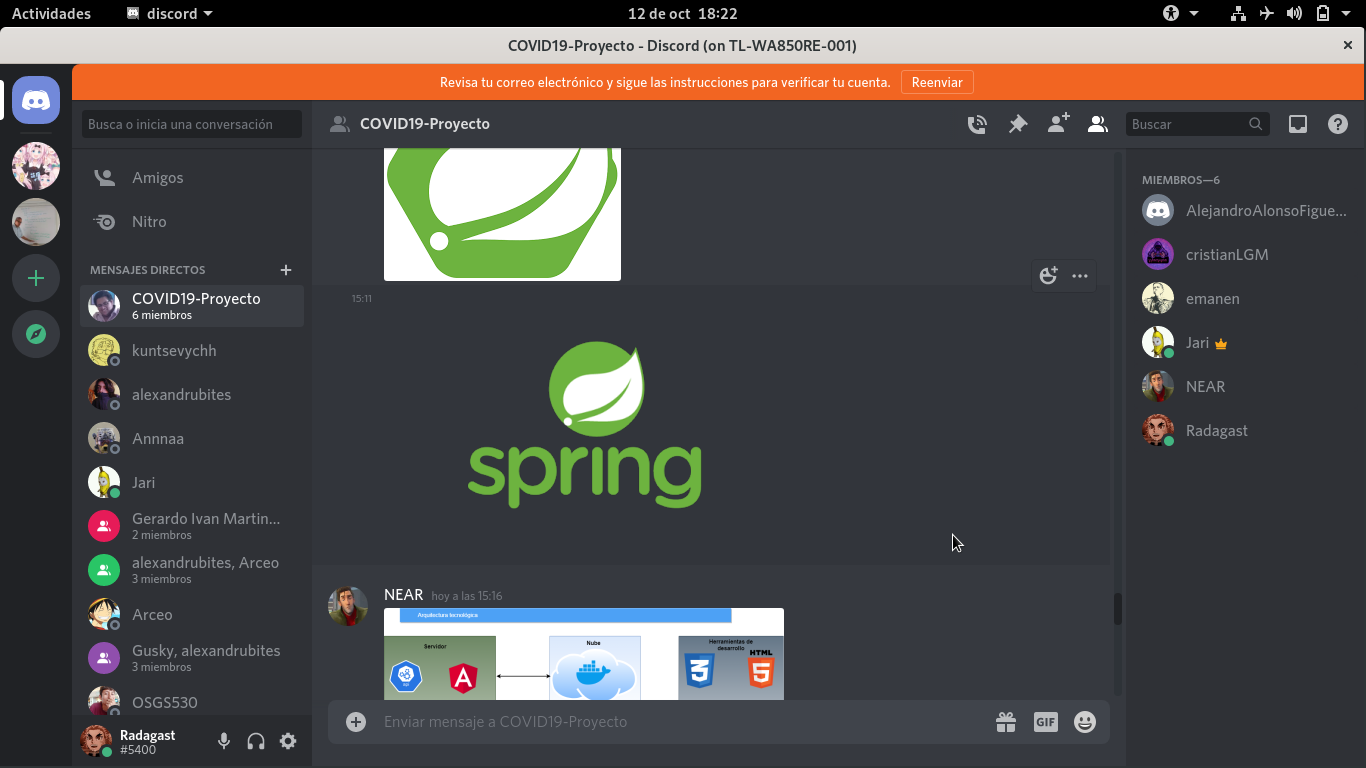
\includegraphics[scale=0.3]{Captura de pantalla de 2020-10-12 18-22-20.png} 

\caption{Captura de pantalla de nuestro grupo de Discord}
\label{fig:captura}
\end{figure}

\end{verse}
 

\end{document}